%% -*- coding: utf-8 -*-
\documentclass{beamer}

%% -*- coding: utf-8 -*-
\usetheme{Boadilla} % default
\useoutertheme{infolines}
\setbeamertemplate{navigation symbols}{} 

\usepackage{etex}
\usepackage{alltt}
\usepackage{pifont}
\usepackage{color}
\usepackage[utf8]{inputenc}
%\usepackage{german}
\usepackage{listings}
\definecolor{keywordcolor}{rgb}{0.7,0.1,0.1}
\definecolor{tacticcolor}{rgb}{0.0,0.1,0.6}
\definecolor{commentcolor}{rgb}{0.4,0.4,0.4}
\definecolor{symbolcolor}{rgb}{0.0,0.1,0.6}
\definecolor{sortcolor}{rgb}{0.1,0.5,0.1}
\definecolor{attributecolor}{rgb}{0.7,0.1,0.1}

\def\lstlanguagefiles{lstlean.tex}
\lstset{language=Lean}
\lstset{sensitive=true}
\usepackage{hyperref}
\hypersetup{colorlinks=true}
\usepackage[final]{pdfpages}
\usepackage{url}
\usepackage{arydshln} % dashed lines
\usepackage{tikz}
\usepackage{mathpartir}

\DeclareUnicodeCharacter{3BB}{\ensuremath{\lambda}}


\newcommand\cmark{\ding{51}}
\newcommand\xmark{\ding{55}}

\newcommand{\nat}{\mathbf{N}}

\usepackage[all]{xy}

%% new arrow tip for xy
\newdir{|>}{!/4.5pt/@{|}*:(1,-.2)@^{>}*:(1,+.2)@_{>}}

\newcommand\cid[1]{\textup{\textbf{#1}}} % class names
\newcommand\kw[1]{\textup{\textbf{#1}}}  % key words
\newcommand\tid[1]{\textup{\textsf{#1}}} % type names
\newcommand\vid[1]{\textup{\texttt{#1}}} % value names
\newcommand\Mid[1]{\textup{\texttt{#1}}} % method names

\newcommand\TODO[1][]{{\color{red}{\textbf{TODO: #1}}}}

\newcommand\String[1]{\texttt{\dq{}#1\dq{}}}

\newcommand\ClassHead[1]{%
  \ensuremath{\begin{array}{|l|}
      \hline
      \cid{#1}
      \\\hline
    \end{array}}}
\newcommand\AbstractClass[2]{%
  \ensuremath{\begin{array}{|l|}
      \hline
      \cid{\textit{#1}}
      \\\hline
      #2
      \hline
    \end{array}}}
\newcommand\Class[2]{%
  \ensuremath{\begin{array}{|l|}
      \hline
      \cid{#1}
      \\\hline
      #2
      \hline
    \end{array}}}
\newcommand\Attribute[3][black]{\textcolor{#1}{\Param{#2}{#3}}\\}
\newcommand\Methods{\hline}
\newcommand\MethodSig[3]{\Mid{#2} (#3): \,\tid{#1}\\}
\newcommand\CtorSig[2]{\Mid{#1} (#2)\\}
\newcommand\AbstractMethodSig[3]{\Mid{\textit{#2}} (#3): \,\tid{#1}\\}
\newcommand\Param[2]{\vid{#2}:~\tid{#1}}

\lstset{%
  frame=single,
  xleftmargin=2pt,
  stepnumber=1,
  numbers=left,
  numbersep=5pt,
  numberstyle=\ttfamily\tiny\color[gray]{0.3},
  belowcaptionskip=\bigskipamount,
  captionpos=b,
  escapeinside={*'}{'*},
  % language=java,
  tabsize=2,
  emphstyle={\bf},
  commentstyle=\mdseries\it,
  stringstyle=\mdseries\rmfamily,
  showspaces=false,
  showtabs=false,
  keywordstyle=\bfseries,
  columns=fullflexible,
  basicstyle=\footnotesize\CodeFont,
  showstringspaces=false,
  morecomment=[l]\%,
  rangeprefix=////,
  includerangemarker=false,
}

\newcommand\CodeFont{\sffamily}

\definecolor{lightred}{rgb}{0.8,0,0}
\definecolor{darkgreen}{rgb}{0,0.5,0}
\definecolor{darkblue}{rgb}{0,0,0.5}

\newcommand\highlight[1]{\textcolor{blue}{\emph{#1}}}
\newcommand\GenClass[2]{\cid{#1}\texttt{<}\cid{#2}\texttt{>}}

\newcommand\Colored[3]{\alt<#1>{\textcolor{#2}{#3}}{#3}}

\newcommand\nt[1]{\ensuremath{\langle#1\rangle}}

\newcommand{\free}{\operatorname{free}}
\newcommand{\bound}{\operatorname{bound}}
\newcommand{\var}{\operatorname{var}}
\newcommand\VSPBLS{\vspace{-\baselineskip}}

\newcommand\IF{\textit{IF}}
\newcommand\TRUE{\textit{TRUE}}
\newcommand\FALSE{\textit{FALSE}}

\newcommand\IFZ{\textit{IF0}}
\newcommand\ZERO{\textit{ZERO}}
\newcommand\SUCC{\textit{SUCC}}
\newcommand\ADD{\textit{ADD}}
\newcommand\SUB{\textit{SUB}}
\newcommand\MULT{\textit{MULT}}
\newcommand\DIV{\textit{DIV}}

\newcommand\PAIR{\textit{PAIR}}
\newcommand\FST{\textit{FST}}
\newcommand\SND{\textit{SND}}

\newcommand\CASE{\textit{CASE}}
\newcommand\LEFT{\textit{LEFT}}
\newcommand\RIGHT{\textit{RIGHT}}

\newcommand\Encode[1]{\lceil#1\rceil}
\newcommand\Reduce{\stackrel\ast\rightarrow_\beta}

\newcommand\Nat{\textit{Nat}}
\newcommand\Bool{\textit{Bool}}
\newcommand\Pair{\textit{Pair}}
\newcommand\Tfun[1]{#1\to}

\newcommand\Tenv{A}
\newcommand\Lam[1]{\lambda#1.}
\newcommand\App[1]{#1\,}
\newcommand\Succ{\textit{SUCC}\,}
\newcommand\Let[2]{\textit{let}\,#1=#2\,\textit{in}\,}

\newcommand\calE{\mathcal{E}}
\newcommand\calU{\mathcal{U}}
\newcommand\calP{\mathcal{P}}
\newcommand\calW{\mathcal{W}}

\newcommand\GEN{\textit{gen}}
\newcommand\EFV[1]{\textit{fv} (#1)}
\newcommand\Dom[1]{\textit{dom} (#1)}

%%% Local Variables: 
%%% mode: latex
%%% TeX-master: nil
%%% End: 

%%% frontmatter
%% -*- coding: utf-8 -*-

\title{Functional Programming / Lean}
\subtitle{Introduction}

\author[Peter Thiemann]{Prof. Dr. Peter Thiemann}
\institute[Univ. Freiburg]{Albert-Ludwigs-Universität Freiburg, Germany}
\date{WS 2026/27}


\subtitle{Type Classes --- Overloading in Lean}
\usepackage{tikz}


\begin{document}

\begin{frame}
  \titlepage
\end{frame}
%----------------------------------------------------------------------
\begin{frame}[fragile]
  \frametitle{Overloading}
  \begin{block}<+->{Remember previous classes?}
    We were able to use
    \begin{itemize}
    \item equality \texttt{==} and ordering \texttt{<} with many different types
    \item arithmetic operations with many different types
    \end{itemize}
  \end{block}
  \begin{block}<+->{Overloading}
    The \textbf{same operator} can be used to execute \textbf{different code} at \textbf{many different types}. 
  \end{block}
  \onslide<+->{Contrast with }
  \begin{block}<+->{Parametric polymorphism}
    The \textbf{same code} can execute at \textbf{many different types}.
  \end{block}
\end{frame}
%----------------------------------------------------------------------
\begin{frame}[fragile]
  \frametitle{Lean integrates overloading with polymorphism}
  \begin{block}<+->{Constrained polymorphism}
    \begin{itemize}
    \item Some functions work on parametric types, but are constrained to specific instances
    \item Types contain type variables and \textbf{constraints}
    \end{itemize}
  \end{block}
  \begin{block}<+->{Examples}
\begin{lstlisting}
-- elem x xs : is x an element of list xs?
-- type a must have equality
List.elem {α : Type} [BEq α] (a : α) (l : List α) : Bool
-- insertSorted x xs : insert x into sorted list xs
-- type a must have comparison
insertSorted : [LE α] → [DecidableLE α] → α → List α → List α
-- square x : compute the square of x
-- type α has multiplication
square : [Mul α] → α → α
\end{lstlisting}
  \end{block}
\end{frame}
%----------------------------------------------------------------------
\begin{frame}[fragile]
  \frametitle{Type classes}
  \begin{itemize}
  \item Each constraint mentions a \textbf{type class}\\
    like \texttt{BEq}, \texttt{LE}, \texttt{Mul}, \dots
  \item A type class specifies a set of operations for a type\\
    e.g.\ \texttt{BEq} requires an operator \texttt{beq}
  \item Type classes form a hierarchy\\
    e.g.\ \lstinline{LawfulBEq (α : Type) [BEq α] : Prop extends ReflBEq α}
  \item Many classes are predefined, but you can roll your own
  \end{itemize}
\end{frame}
%----------------------------------------------------------------------
\begin{frame}[fragile]
  \frametitle{Classes and Instances}
  \begin{itemize}
  \item A \emph{class declaration} specifies a signature (i.e., the class members and their types)
\begin{lstlisting}
class Monoid (α : Type) where
  op : α → α → α
  id : α
\end{lstlisting}
  \item An \emph{instance declaration} specifies that a type belongs to a class by giving definitions for all class members
\begin{lstlisting}
instance MonoidInt : Monoid Int where
  op := Int.add
  id := 0
\end{lstlisting}
  \item This info can be obtained from Lean by
\begin{lstlisting}
#print Monoid
\end{lstlisting}
  \end{itemize}
\end{frame}
\begin{frame}[fragile]
  \frametitle{Defining \texttt{Monoid} for pairs}
\begin{lstlisting}
instance MonoidPair [Monoid α][Monoid β] : Monoid (α × β) where
  op := fun (x1, y1) (x2, y2) => (Monoid.op x1 x2, Monoid.op y1 y2)
  id := (Monoid.id, Monoid.id)
\end{lstlisting}
  \begin{itemize}
  \item Instance can have any number of assumptions / constraints on the type
    variables.
  \item Definition is \textbf{not} recursive!
  \end{itemize}
\end{frame}
%----------------------------------------------------------------------
\begin{frame}[fragile,fragile]
  \frametitle{Groups extend monoids}
\begin{lstlisting}
class Group (α : Type) extends Monoid α where
  inv : α → α

instance GroupInt : Group Int where
  inv := Int.neg

instance GroupPair [Group α][Group β] : Group (α × β) where
  inv := fun (x, y) => (Group.inv x, Group.inv y)
\end{lstlisting}
  \begin{itemize}
  \item requires the \lstinline{MonoidInt} instance
  \item requires the \lstinline{MonoidPair} instance
  \item extension means:\\ can use instances of \lstinline{Group} where instances
    of \lstinline{Monoid} is required 
  \end{itemize}
\end{frame}
%----------------------------------------------------------------------
\begin{frame}[fragile]
  \frametitle{Further useful classes}
  \begin{block}<+->{ToString and Repr}
\begin{lstlisting}
class ToString (α : Type) where
  toString : α → String

class Repr (α : Type) where
  reprPrec : α → Nat → Std.Format
\end{lstlisting}
    \begin{itemize}
    \item \lstinline{Repr} is predefined for most built-in types
    \item Derivable for most datatype definitions
    \end{itemize}
  \end{block}
\end{frame}
%----------------------------------------------------------------------
\begin{frame}[fragile]
  \frametitle{Handwriting vs deriving an instance}
  \begin{block}<+->{Remember the Hearts game}
\begin{lstlisting}
inductive Color where
  | red
  | black

instance : ToString Color where
  toString
    | .red => "red"
    | .black => "black"

instance : BEq Color where
  beq
    | .red, .red => true
    | .black, .black => true
    | _, _ => false
\end{lstlisting}
  \end{block}
\end{frame}
%----------------------------------------------------------------------
\begin{frame}[fragile]
  \frametitle{The \texttt{Ord} class (derivable)}
\begin{lstlisting}
inductive Ordering where
  | lt | eq | gt

class Ord (α : Type) where
  compare : α → α → Ordering
\end{lstlisting}
  Different from \lstinline{LE} and \lstinline{LT}!
\end{frame}
%----------------------------------------------------------------------
\begin{frame}[fragile]
  \frametitle{Equality}
  \begin{block}<+->{The type class \texttt{BEq}}
\begin{lstlisting}
class BEq (α : Type)  where
  beq : α → α -> Bool
infix:50 " == " => BEq.beq

def bne [BEq α] (x y : α) : Bool :=
  !(x == y)
infix:50 " != " => bne
\end{lstlisting}
  \end{block}
  \begin{itemize}
  \item Equality is special because Lean also supports proof
  \item Distinguish
    \begin{itemize}
    \item \emph{boolean equality} \lstinline{beq} for programming
    \item \emph{propositional equality} \lstinline{=} for proving
    \end{itemize}
  \item They are connected
  \end{itemize}
\end{frame}
%----------------------------------------------------------------------
\begin{frame}[fragile]
  \frametitle{Logical backing for equality}
\begin{lstlisting}
class ReflBEq (α) [BEq α] : Prop where
  protected rfl {a : α} : a == a
\end{lstlisting}

  \begin{itemize}
  \item Constrained to members of \lstinline{BEq}
  \item Contains the logical proposition $\forall a. a == a$ (reflexivity)
  \item Instantiating \lstinline{ReflBEq} requires \emph{proof} of this proposition.
  \end{itemize}
  
\begin{lstlisting}
class LawfulBEq (α : Type u) [BEq α] : Prop extends ReflBEq α where
  eq_of_beq : {a b : α} → a == b → a = b
\end{lstlisting}
  \begin{itemize}
  \item extends: Can use \lstinline{LawfulBEq} instances where
    \lstinline{ReflBEq} is required
  \item \lstinline{eq_of_beq} says that boolean equality implies propositional
    equality.
  \item In this context \lstinline{a == b} stands for \lstinline{(a == b) = true}!
  \item Instantiating also requires proof.
  \end{itemize}
  
\end{frame}
% ----------------------------------------------------------------------
\begin{frame}
  \frametitle{Equality}
  \begin{block}<+->{Flavors of equality \dots}
    What does $a = b$ mean?
  \end{block}
  \begin{block}<+->{Propositional equality}
    There is a proof that $a$ and $b$ are equal.
  \end{block}
  \begin{block}<+->{Definitional equality}
    $a$ and $b$ evaluate to the same result.

    (by applying definitions)

    Here the proof for $a = b$ is by \emph{reflexivity}.
  \end{block}
  \begin{block}<+->{}\scalebox{0.8}{
    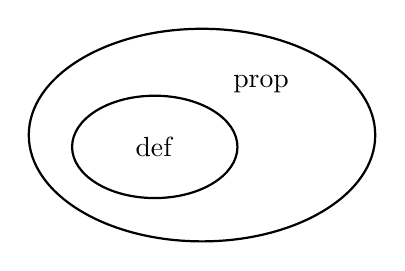
\begin{tikzpicture}
  \draw[thick] (0,0) ellipse (2.2cm and 1.35cm);
  \draw[thick] (-0.6,-0.15) ellipse (1.05cm and 0.65cm);

  \node at (-0.6,-0.15) {$\mathrm{def}$};
  \node at (0.75,0.65) {$\mathrm{prop}$};
\end{tikzpicture}}
  \end{block}
\end{frame}
%----------------------------------------------------------------------
\begin{frame}[fragile,fragile]
  \frametitle{Defining propositional equality}
  Another inductive datatype
\begin{lstlisting}
inductive Eq (x : α) : α → Prop where
  | refl : Eq x x
\end{lstlisting}
  Propositional equality is an equivalence relation
\begin{lstlisting}
theorem symEq : ∀ {x y : α}, Eq x y → Eq y x :=
  fun h =>
  match h with
  | Eq.refl => Eq.refl

theorem transEq : ∀ {x y z : α}, Eq x y → Eq y z → Eq x z :=
  fun h1 h2 =>
  match h1, h2 with
  | Eq.refl, Eq.refl => Eq.refl
\end{lstlisting}
  \begin{alertblock}{}
    Lean wraps the \lstinline{Eq.refl} constructor in \lstinline{rfl}.
  \end{alertblock}
\end{frame}
%----------------------------------------------------------------------
\begin{frame}[fragile]
  \frametitle{Excursion on proofs}
  \framesubtitle{Propositions and proofs}
  \begin{exampleblock}<+->{Examples}
\begin{lstlisting}
2 * 3 = 6
Sorted [1,2,3]
insertSorted 2 [1, 3] = [1, 2, 3]
\end{lstlisting}
  \end{exampleblock}
  \vspace{-0.5\baselineskip}
  \begin{block}<+->{Proof by tactic}
\begin{lstlisting}
theorem easyDef1 : 4 + 5 = 9 := by rfl
\end{lstlisting}
    \lstinline{4 + 5} and \lstinline{9} are \emph{definitionally equal}, so the
    proposition is true by reflexivity of equality. Using tactic \lstinline{rfl}
    preceded by keyword \lstinline{by}.
  \end{block}
  \vspace{-0.5\baselineskip}
  \begin{block}<+->{Proof by proof term}
\begin{lstlisting}
theorem easyDef0 : 2 * 3 = 6 := eq_of_beq (BEq.refl 6)
\end{lstlisting}
    \begin{itemize}
    \item \lstinline{BEq.refl 6} gives \lstinline{(6 == 6) = true}
    \item \lstinline{eq_of_beq} yields the required \lstinline{6 = 6}
    \end{itemize}
  \end{block}
\end{frame}
%----------------------------------------------------------------------
\begin{frame}[fragile,fragile]
  \frametitle{Defining propositions}
  \framesubtitle{Propositions behave like values}
  \begin{block}<+->{A provable proposition}
\begin{lstlisting}
def prop1 : Prop := 3 + 4 = 7
theorem prop1_is_true : prop1 := rfl
\end{lstlisting}
  \end{block}
  \begin{block}<+->{A false proposition}
\begin{lstlisting}
def prop2 : Prop := 3 + 4 = 8
\end{lstlisting}
  \end{block}
  \begin{block}<+->{Another provable proposition}
\begin{lstlisting}
theorem prop3_thm : 3 ≤ 4 := by
  decide
\end{lstlisting}
    Tactic \lstinline{decide} invokes a \emph{decision procedure} that (in this
    case) constructs a proof for \lstinline{3 ≤ 4}. It only works with concrete
    arguments.
  \end{block}
\end{frame}
%----------------------------------------------------------------------
\begin{frame}[fragile,fragile]
  \frametitle{Building blocks of propositions}
  \framesubtitle{The logical connectives}
  ``And'' and ``Or'' definable using inductives
\begin{lstlisting}
inductive And (p q : Prop) : Prop where
  | intro : p → q → And p q

inductive Or (p q : Prop) : Prop where
  | inl : p → Or p q
  | inr : q → Or p q
\end{lstlisting}
  There are syntax definitions for $p \wedge q$ and $p\vee q$.

\begin{lstlisting}
theorem and1 : 1 + 1 = 2 ∧ 2 + 2 = 4 := by decide  -- rfl does not work
theorem or1 : 1 + 1 = 2 ∨ 2 + 2 = 5 := by decide   -- rfl does not work
theorem and2 : 1 + 1 = 2 ∧ 2 + 2 ≤ 5 := by decide
\end{lstlisting}
Combinations of decidable propositions are also decidable.
\end{frame}
%----------------------------------------------------------------------
\begin{frame}[fragile]
  \frametitle{Some simple theorems}
  \begin{block}<+->{Proof by giving a proof term of suitable type}
\begin{lstlisting}
theorem and_comm {p q : Prop} : p ∧ q → q ∧ p :=
  fun pq =>
  match pq with
  | .intro left right => .intro right left
\end{lstlisting}
  \end{block}
  \begin{block}<+->{Proof by tactics}
\begin{lstlisting}
theorem and_comm' {p q : Prop} : p ∧ q → q ∧ p := by
  intro pq
  exact .intro pq.right pq.left
\end{lstlisting}
    \begin{itemize}
    \item Tactic \lstinline{intro pq} makes \lstinline{p ∧ q} an assumption and
      \lstinline{q ∧ p} the goal
    \item Tactic \lstinline{exact} switches to proof term mode
    \end{itemize}
  \end{block}
\end{frame}
%----------------------------------------------------------------------
\begin{frame}[fragile]
  \frametitle{Application: Indexing}
  \begin{block}<+->{Example}
\begin{lstlisting}
def bassists : List String := ["Geddy Lee", "John Myung", "Chris Squire"]

def john_myung : String := bassists[1]
#eval john_myung
def chris_squire : String := bassists[2]
#eval chris_squire
def morty : String := bassists[3] -- Error because index is out of bounds
#eval! morty
\end{lstlisting}
  \end{block}
  \begin{alertblock}<+->{Error}\small
\begin{verbatim}
failed to prove index is valid, possible solutions:
  - Use `have`-expressions to prove the index is valid
  - Use `a[i]!` notation instead, runtime check is performed, and 'Panic' error message is produced if index is not valid
  - Use `a[i]?` notation instead, result is an `Option` type
  - Use `a[i]'h` notation instead, where `h` is a proof that index is valid
|- 3 < bassists.lengthLean 4
\end{verbatim}
  \end{alertblock}
\end{frame}
%----------------------------------------------------------------------
\begin{frame}[fragile,fragile]
  \frametitle{Safe Indexing}
  \begin{alertblock}<+->{Not accepted}
\begin{lstlisting}
def third {α } (xs : List α) : α := xs[2]
\end{lstlisting}
  \end{alertblock}

  \begin{exampleblock}<+->{Ok}
\begin{lstlisting}
def third {α} (xs : List α) (h : xs.length > 2) : α := xs[2]

#eval third bassists (by decide)
\end{lstlisting}
  \end{exampleblock}
\end{frame}
%----------------------------------------------------------------------
\begin{frame}[fragile]
 \frametitle{Inductive Propositions}
  \begin{block}<+->{An inductive proposition}
\begin{lstlisting}
inductive Sorted [LE α] : List α → Prop where
  | nil : Sorted []
  | cons : ∀ {x xs}, Sorted xs → (∀ y ∈ xs, x ≤ y) → Sorted (x :: xs)

def Sorted123 : Prop := Sorted [1, 2, 3]
\end{lstlisting}
  \end{block}
\end{frame}
%----------------------------------------------------------------------
% \begin{frame}[fragile]
%   \frametitle{Defining \texttt{Eq} for pairs}
%   \begin{block}<+->{When are two pairs equal?}
%   \end{block}
%   \begin{block}<+->{Solution}
% \begin{lstlisting}
% instance (Eq a, Eq b) => Eq (a, b) where
%   (a1, b1) == (a2, b2) = a1 == a2 && b1 == b2
% \end{lstlisting}
%   \end{block}
%   \begin{block}<+->{Is this definition recursive?}
%   \end{block}
%   \begin{alertblock}<+->{YES: on types, NO: on values}
%   \end{alertblock}
% \end{frame}
%----------------------------------------------------------------------
% \begin{frame}[fragile]
%   \frametitle{Defining \texttt{Eq} for lists}
%   \begin{block}<+->{When are two lists equal?}
%   \end{block}
%   \begin{block}<+->{Solution}
% \begin{lstlisting}
% instance Eq a => Eq [a] where
%   [] == [] = True
%   (x:xs) == (y:ys) = x == y && xs == ys
%   _ == _ = False
% \end{lstlisting}
%   \end{block}
%   \begin{block}<+->{Is this definition recursive?}
%   \end{block}
%   \begin{alertblock}<+->{YES: on types, YES: on values}
%     The equality \texttt{xs == ys}.
%   \end{alertblock}
% \end{frame}
%----------------------------------------------------------------------
%----------------------------------------------------------------------
% \begin{frame}[fragile]
%   \frametitle{More classes for you to investigate}
%   \begin{itemize}
%   \item \texttt{Enum} (derivable)
%   \item \texttt{Bounded} (derivable)
%   \end{itemize}
% \begin{lstlisting}
% \end{lstlisting}
% \end{frame}
%----------------------------------------------------------------------
% \begin{frame}[fragile]
%   \frametitle{Ambiguity}
% \onslide<+->{Some combinations of overloaded functions can lead to ambiguity}
% \begin{lstlisting}
% f x = read (show x)
% g x = show (read x)
% \end{lstlisting}
% \begin{block}<+->{What are types of \texttt{f} and \texttt{g}?}
% \end{block}
% \begin{block}<+->{Solution}
% \begin{lstlisting}
% f : (Read a, Show b) => b -> a
% g : String -> String
% \end{lstlisting}
% \end{block}
% \end{frame}
%----------------------------------------------------------------------
% \begin{frame}[fragile]
%   \frametitle{Further pitfalls / features}
%   \begin{itemize}
%   \item Definitions without arguments and without type signatures are not overloaded (monomorphism restriction)
%   \item Numeric literals are overloaded at type \texttt{Num a => a}
%   \item Haskell has a \textbf{defaulting} mechanism that resolves violations of the monomorphism restriction 
%   \item Caveat: GHCi behaves differently than code in a file
%   \end{itemize}
% \end{frame}
%----------------------------------------------------------------------
%----------------------------------------------------------------------
\begin{frame}
  \frametitle{Wrapup}
  \begin{alertblock}{Type classes}
  \begin{itemize}
  \item provide a signature for an abstract data type
  \item instances provide implementations at unrelated types
  \item many classes are predefined and derivable
  \item pervasively used in Lean
  \end{itemize}
  \end{alertblock}
\end{frame}

% \begin{frame}
%   \frametitle{Break Time --- Questions?}
%   \begin{center}
%     \tikz{\node[scale=15] at (0,0){?};}
%   \end{center}
% \end{frame}


\end{document}

%%% Local Variables: 
%%% mode: latex
%%% TeX-master: t
%%% End: 
